
\begin{lemma}{7.2.285}\label{lem:7-2-285}
存在 $[0,1]^2\times L'_1$ 的光滑奇异链复形的
一个可数生成子复形
\[
C_X([0,1]^2\times L'_1,(\lambda_0,\lambda'_1)),
\]
它带有滤过 $A_{n',K'}$ 代数结构，
以及下列滤过 $A_{n',K'}$ 同态：
\begin{equation}
\begin{aligned}
\operatorname{Eval}_{r=r_0}\colon
C_X([0,1]^2\times L'_1,(\lambda_0,\lambda'_1))
&\longrightarrow
C^{r=r_0}([0,1]_s\times L'_1,(\lambda_0,\lambda'_1)),\\
\operatorname{Eval}_{s=s_0}\colon
C_X([0,1]^2\times L'_1,(\lambda_0,\lambda'_1))
&\longrightarrow
C^{s=s_0}([0,1]_r\times L'_1,(\lambda_0,\lambda'_1)),
\end{aligned}
\tag{7.2.286.1}\label{eq:7-2-286-1}
\end{equation}
\begin{equation}
\operatorname{Incl}\colon C(L'_1,\lambda'_1)
\longrightarrow C_X([0,1]^2\times L'_1,(\lambda_0,\lambda'_1)),
\tag{7.2.286.2}\label{eq:7-2-286-2}
\end{equation}
还有滤过 $A_{n,K}$ 同态
\begin{equation}
\mathfrak f^{\{\Phi_{r,s}\}_{r,s}}\colon
C(L_0,\lambda_0)
\longrightarrow C_X([0,1]^2\times L'_1,(\lambda_0,\lambda'_1)),
\tag{7.2.286.3}\label{eq:7-2-286-3}
\end{equation}
满足以下性质：

\par\noindent\textup{(7.2.287.1)}
$\operatorname{Eval}$ 与 $\operatorname{Incl}$
满足 (7.2.189.1)--(7.2.189.7)。

\par\noindent\textup{(7.2.287.2)}
有
\[
\begin{aligned}
\operatorname{Eval}_{r=r_0}\circ
\mathfrak f^{\{\Phi_{r,s}\}_{r,s}}
&=\mathfrak f^{\{\Phi_{r_0,s}\}_s},\\
\operatorname{Eval}_{s=s_0}\circ
\mathfrak f^{\{\Phi_{r,s}\}_{r,s}}
&=\mathfrak f^{\{\Phi_{r,s_0}\}_r}.
\end{aligned}
\]
\end{lemma}

\par\noindent\textit{证明.}\quad
这是第 7.2.10 小节（命题 7.2.160、7.2.162）的
双参数版本。先定义
$C_X([0,1]^2\times L'_1,(\lambda_0,\lambda'_1))$。
为此考虑定义 4.6.30 的双参数版本。
从这里到本小节末，花体字母 $\mathfrak P$ 等
表示 $[0,1]^2\times L'_1$ 上的光滑奇异单形。

\begin{definition}{7.2.288}\label{def:7-2-288}
设 $\mathfrak P=(|\mathfrak P|,f)$ 是光滑奇异单形，
$f\colon|\mathfrak P|\to[0,1]^2\times L'_1$。
若对 $s_0,r_0=0,1$ 均满足以下条件，
则称 $\mathfrak P$ 为\emph{适配奇异单形}\liftIndex{I278}：

\par\noindent\textup{(7.2.289.1)}
$f^{-1}(\{r_0\}\times[0,1]_s\times L'_1)
\cap|\mathfrak P|$
或为空，或恰由一个面（余维任意）组成，
或等于 $|\mathfrak P|$ 本身。
对于 $f^{-1}([0,1]_r\times\{s_0\}\times L'_1)
\cap|\mathfrak P|$ 同样成立。

\par\noindent\textup{(7.2.289.2)}
$f^{-1}(\{r_0\}\times\{s_0\}\times L'_1)
\cap|\mathfrak P|$
或为空，或恰由一个余维任意的面组成，
或等于 $|\mathfrak P|$ 本身。

\par\noindent\textup{(7.2.289.3)}
设 $\Delta_c^m$ 是 $|\mathfrak P|$ 的任意余维的面，
且 $f(\Delta_c^m)$ 与角点
$\{r_0\}\times\{s_0\}\times L'_1$ 相交。
则以下二者之一成立：
\begin{enumerate}[label=\textup{(\roman*)},leftmargin=3.5em]
\item $f(\Delta_c^m)$ 包含于边界分量
$\{r_0\}\times[0,1]_s\times L'_1$
或 $[0,1]_r\times\{s_0\}\times L'_1$ 中；
\item $f(\Delta_c^m)$ 同时与
$\{r_0\}\times(0,1)_s\times L'_1$ 和
$(0,1)_r\times\{s_0\}\times L'_1$ 相交。
\end{enumerate}

\par\noindent\textup{(7.2.289.4)}
若 $f^{-1}(\{0\}\times[0,1]_s\times L'_1)
\cap|\mathfrak P|$ 非空，则
\[
f(|\mathfrak P|)\subset
[0,1/3)_r\times[0,1]_s\times L'_1.
\]
若 $f^{-1}(\{1\}\times[0,1]_s\times L'_1)
\cap|\mathfrak P|$ 非空，则
\[
f(|\mathfrak P|)\subset
(2/3,1]_r\times[0,1]_s\times L'_1.
\]
对 $s$ 坐标也有同样条件。

\par\noindent\textup{(7.2.289.5)}
设 $\Delta_a^m$ 是 $|\mathfrak P|$ 的一个面，
$\Delta_b^{m'}$ 是包含它的另一个面。
若 $\Delta_a^m\subset
f^{-1}(\{r_0\}\times[0,1]_s\times L'_1)$，
而 $\Delta_b^{m'}$ 不包含于此逆像，
则对 $x\in\Delta_a^m$ 及任意
$N\in T_x\Delta_b^{m'}\setminus
T_x(\partial\Delta_b^{m'})$，
$f_*(N)$ 的 $[0,1]_r$ 分量非零。
对 $s$ 坐标同样成立。
\translatornote{原书此条件第一处端面逆像将
$[0,1]_s$ 与 $L'_1$ 之间的乘号误排为逗号；
此处按同条件紧接的第二处逆像及 (7.2.289.1) 写乘积。}
\end{definition}

例如，图~\ref{fig:7-2-13} 的三角形 (1) 适配，
三角形 (2) 不适配。
\par\medskip\noindent\begin{minipage}{\textwidth}
\centering
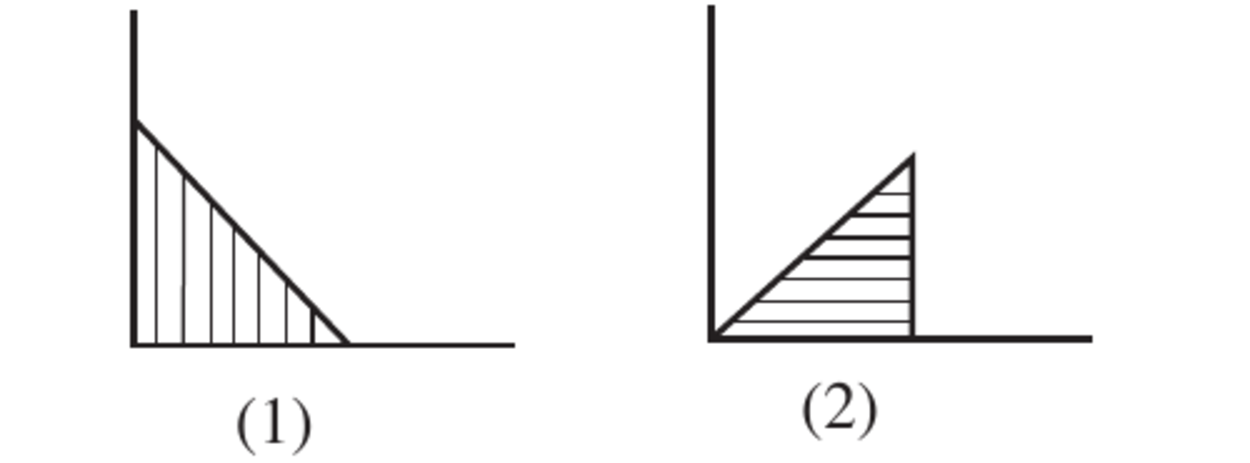
\includegraphics[width=.52\textwidth]{chapters/ch07-transversality/figures/phys-550-figure-7-2-13-math2-crop.png}
\par{\renewcommand{\thefigure}{7.2.13}\refstepcounter{figure}
\normalfont\bfseries 图~\thefigure\label{fig:7-2-13}}
\end{minipage}\par\medskip

令 $S_+([0,1]^2\times L'_1)$ 是由适配奇异单形
自由生成的阿贝尔群。显然它是
$[0,1]^2\times L'_1$ 的奇异链复形的子复形。
定义商复形
\[
S([0,1]^2\times L'_1)
=\frac{S_+([0,1]^2\times L'_1)}
{S_+([0,1]^2\times L'_1)
\cap S(\partial([0,1]^2\times L'_1))},
\]
分母是由包含于
$\partial([0,1]^2\times L'_1)$ 的适配单形
生成的子复形。维数为 $m$ 的奇异链
$\mathfrak P$ 的次数为
\[
d=\dim L'_1+2-m.
\]

现在定义评价映射
\[
\operatorname{Eval}_{s=s_0}\colon
S([0,1]^2\times L'_1)
\longrightarrow S([0,1]_r\times L'_1).
\]
若 $f^{-1}([0,1]_r\times\{s_0\}\times L'_1)
\cap|\mathfrak P|$ 在 $|\mathfrak P|$ 中
不是余维一，则令
$\operatorname{Eval}_{s=s_0}(\mathfrak P)=0$。
若它是第 $c$ 个余维一的面，则令
\[
\operatorname{Eval}_{s=s_0}(\mathfrak P)
=(-1)^{s_0+c}(\Delta_c^{m-1},f_c\circ j_c),
\]
其中
$\Delta_c^{m-1}=(v_0,\ldots,\widehat v_c,\ldots,v_m)$
就是该逆像面，
$f_c=f|_{\Delta_c^{m-1}}$，
$j_c\colon\Delta^{m-1}\to\Delta_c^{m-1}$
由
\[
j_c(v_i)=
\begin{cases}
v_i,&i<c,\\
v_{i+1},&i\ge c
\end{cases}
\]
给出。
\translatornote{原书在此再次把 $j_c$ 第二分支写作
$i>c$，从而漏掉 $v_c$ 的像；
按 A-0452 已裁决的删点面嵌入读作 $i\ge c$。}
这里已计入交换映射
$[0,1]_r\times[0,1]_s\to
[0,1]_s\times[0,1]_r$ 反转定向的事实。

与第 7.2.10 小节相同，定义
$\operatorname{Eval}_{r=r_0}$：
若 $f^{-1}(\{r_0\}\times[0,1]_s\times L'_1)
\cap|\mathfrak P|$ 不是余维一，令
$\operatorname{Eval}_{r=r_0}(\mathfrak P)=0$；
若它是 $\mathfrak P$ 的第 $c$ 个余维一的面，令
\[
\operatorname{Eval}_{r=r_0}(\mathfrak P)
=(-1)^{r_0+c+1}(\Delta^{m-1},f_c\circ j_c).
\]

在同调层次，$\operatorname{Eval}$ 可视为连接同态
\[
\resizebox{\textwidth}{!}{$\displaystyle
\begin{aligned}
H_m([0,1]^2\times L'_1;
\partial([0,1]^2\times L'_1))
&\longrightarrow
\bigoplus_{r_0=0,1}
H_{m-1}(\{r_0\}\times[0,1]_s\times L'_1;
\{r_0\}\times\{0,1\}\times L'_1)\\
&\qquad\oplus
\bigoplus_{s_0=0,1}
H_{m-1}([0,1]_r\times\{s_0\}\times L'_1;
\{0,1\}\times\{s_0\}\times L'_1).
\end{aligned}
$}
\]
它是上同调群之间由包含诱导的映射的庞加莱对偶。
上述链复形的选取，正是为了在链级实现这个同态。

如图~\ref{fig:7-2-14}，把 $[0,1]^2$ 分成
$18$ 个三角形。设
$P=(|P|,f)$ 是 $L'_1$ 的光滑奇异单形。
将 $[0,1]^2\times|P|$ 分成 $18$ 个棱柱，
再把每个棱柱细分为单形。
可以选择这种细分，使
\[
\operatorname{id}\times f\colon
[0,1]^2\times|P|\longrightarrow
[0,1]^2\times L'_1
\]
在每个单形上的限制都适配，
亦即满足定义~\ref{def:7-2-288}。

\par\medskip\noindent\begin{minipage}{\textwidth}
\centering
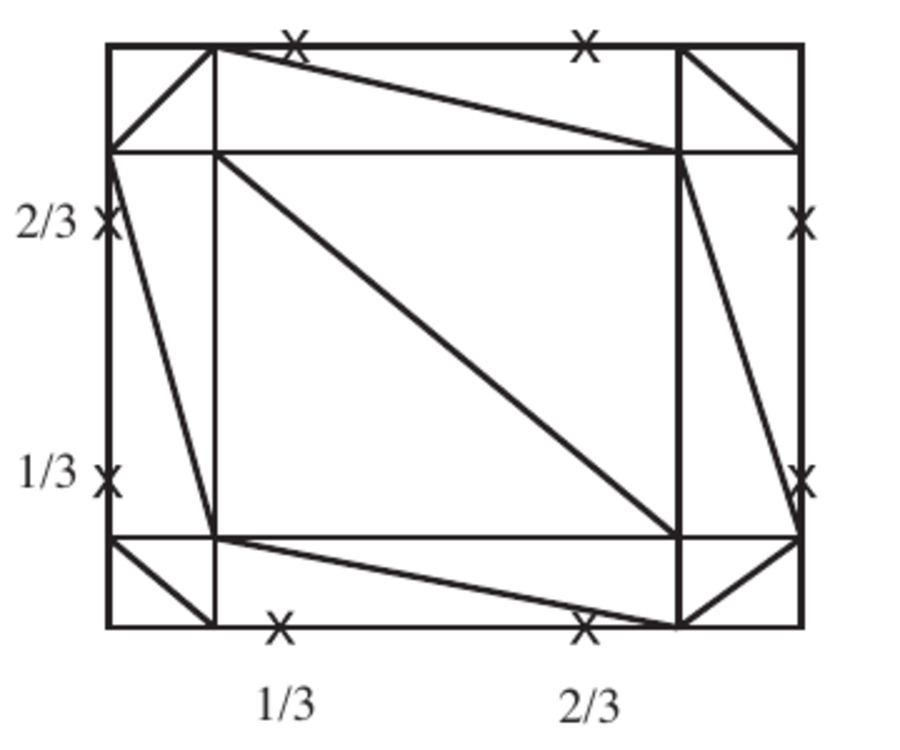
\includegraphics[width=.45\textwidth]{chapters/ch07-transversality/figures/phys-551-figure-7-2-14-math2-crop.png}
\par{\renewcommand{\thefigure}{7.2.14}\refstepcounter{figure}
\normalfont\bfseries 图~\thefigure\label{fig:7-2-14}}
\end{minipage}\par\medskip

把这样得到的最高维奇异单形求和，
定义
$\operatorname{Incl}_{1,\beta_0}(P)
\in S([0,1]^2\times L'_1)$。
由此得到链映射
\[
\operatorname{Incl}_{1,\beta_0}\colon
S(L'_1)\longrightarrow S([0,1]^2\times L'_1).
\]

可以选择 $[0,1]^2\times|P|$ 的细分，使
\begin{equation}
\begin{aligned}
\operatorname{Eval}_{s=s_0}\circ
\operatorname{Incl}_{1,\beta_0}
&=(\operatorname{Incl}_r)_{1,\beta_0},\\
\operatorname{Eval}_{r=r_0}\circ
\operatorname{Incl}_{1,\beta_0}
&=(\operatorname{Incl}_s)_{1,\beta_0}.
\end{aligned}
\tag{7.2.290}\label{eq:7-2-290}
\end{equation}
其中
$(\operatorname{Incl}_r)_{1,\beta_0}\colon
S(L'_1)\to S([0,1]_r\times L'_1)$
与
$(\operatorname{Incl}_s)_{1,\beta_0}\colon
S(L'_1)\to S([0,1]_s\times L'_1)$
定义于 (7.2.135)。

\begin{lemma}{7.2.291}\label{lem:7-2-291}
\par\noindent\textup{(7.2.292.1)}
$\operatorname{Eval}_{r=r_0}$ 和
$\operatorname{Eval}_{s=s_0}$
对 $\mathfrak m_{1,\beta_0}$ 是链映射。

\par\noindent\textup{(7.2.292.2)}
有
$\operatorname{Eval}_{r=r_0}\circ
\operatorname{Eval}_{s=s_0}
=\operatorname{Eval}_{s=s_0}\circ
\operatorname{Eval}_{r=r_0}$；
等式两边都是从
$S([0,1]^2\times L'_1)$ 到 $S(L'_1)$ 的映射。
\translatornote{原书本分项的源、靶孤立地写作
$S([0,1]^2\times L')$、$S(L')$，
本引理及其证明所在模型均为 $L'_1$，故在此补下标。}

\par\noindent\textup{(7.2.292.3)}
$\operatorname{Eval}$ 与
$(\operatorname{Incl})_{1,\beta_0}$
在同调上诱导同构。

\par\noindent\textup{(7.2.292.4)}
为便于排印，记本序列的中项为
\[
D_{\partial}=
\bigoplus_{r_0=0,1}
S(\{r_0\}\times[0,1]_s\times L'_1)
\oplus
\bigoplus_{s_0=0,1}
S([0,1]_r\times\{s_0\}\times L'_1).
\]
则下列序列正合：
\[
S([0,1]^2\times L'_1)
\xrightarrow{A}D_{\partial}
\xrightarrow{B}S(L'_1)^{4\oplus}
\longrightarrow 0.
\]
其中 $A$、$B$ 的定义与 (7.2.189.5) 类似。
\end{lemma}
